%xelatex
%shell-escape для minted
\documentclass[a4paper, 12pt, oneside]{extarticle}
\input{$UNI/.templates/settings/preamble.tex}
\input{$UNI/.templates/settings/font_styles.tex}
\input{$UNI/.templates/settings/minted_settings.tex}
\addbibresource{~/Documents/uni/bibliography.bib}

\usepackage[explicit]{titlesec}
% \usepackage[svgnames]{xcolor}

\renewcommand\Variant{0.168}
% \newcommand\Date{DAY.MONTH.\the\year}
\newcommand\Type{\Lab} % \Lab \Pract \RGR
\Work{num}
% \newcommand\Number{NUMBER}
\newcommand\Topic{Визначення суми \\ послідовності на основі \\ циклічного додавання}

% \titleformat{\section}
% {\color{red}\normalfont\Large\bfseries}
% {\color{red}\thesection}{1em}{}
\usepackage[breakable]{tcolorbox}

\newcommand\tcobx[1]{
\begin{tcolorbox}[breakable, arc=0mm, colback=white, boxrule=0.2mm, beforeafter skip=0pt]
	#1
\end{tcolorbox}
}

% ---
% pdf-engine: xelatex
% header-includes:
% - \input{$UNI/.templates/settings/preamble.tex}
% - \input{$UNI/.templates/settings/minted_settings.tex}
% - \newcommand\Type{\Lab}
% - \Work{num}
% - \renewcommand\Variant{0.168}
% - \newcommand\Date{15.9.\the\year}
% - \newcommand\Number{1}
% - \newcommand\Topic{Визначення суми послідовності на основі циклічного додавання}
% - \usepackage{csvsimple}
% - \usepackage{longtable}
% ---

\usepackage{blindtext}

\titleformat{\section}
[display]
{\color{black}\normalfont\bfseries}
{}
{0pt}
{\begin{tcolorbox}[arc=0mm, colback=blue!10!white, boxrule=0.2mm, beforeafter skip=0pt, boxsep=0mm]{ #1}\end{tcolorbox}}

\titleformat{\subsection}
[display]
{\color{black}\normalfont\bfseries}
{}
{0pt}
{\begin{tcolorbox}[arc=0mm, colback=blue!10!white, boxrule=0.2mm, beforeafter skip=0pt, boxsep=0mm]{ #1}\end{tcolorbox}}

\titlespacing*{\section}{0pt}{0ex}{-4ex}
\titlespacing*{\subsection}{0pt}{0ex}{-4ex}

\usepackage{multirow}
\usepackage{makecell}
\usepackage{tabularx}

\begin{document}

\Margins
%\begin{wrapfigure}[3]{l}{.27\textwidth}
%\includegraphics[width=.28\textwidth]{$UNI/.templates/lpnu_logo.png}
%\end{wrapfigure}

%\noindent\textbf{Прізвище:} \Lname \\
%\noindent\textbf{Ім'я:} \Fname \\
%\noindent\textbf{Група:} \Group \\
%\noindent\textbf{Варіант:} \Variant \\
%\noindent\textbf{Дата захисту:} \Date \\
%\\
%\noindent\textbf{Кафедра:} \Department \\
%\noindent\textbf{Дисципліна:} \Discipline \\
%\noindent\textbf{Перевірив:} \Instructor \\

%%\medskip\bigskip

%\begin{center}
%	\textbf{ЗВІТ}		\\
%	до \Type~\No\Number	\\
%	на тему ``\Topic''	\\
%\end{center}

% \begin{table}
%   \begin{tabularx}{\textwidth}{|c|X|X|}
%     \hline
%     % Image & Content & Additional Info \\
%     % \hline
% 	  \multirow{3}{*}{\includegraphics[width=4cm]{$UNI/.templates/lpnu_logo.png}}
% 	  & \textbf{ЗВО:}
% 	  Національний університет ``Львівська Політехніка''.
% 	  & \textbf{Тема:}
% 	  \Topic
% 	  \\
% 	  & \textbf{Навчальний рік:}
% 	  2023/2024
% 	  & \textbf{Інститут}
% 	  комп'ютерних наук та інформаційних технологій
% 	  \\
% 	  & \textbf{Семестр:}
% 	  осінній
% 	  & \textbf{Група:}
% 	  \Group
% 	  \\
% 	  & \textbf{Навчальна дисципліна:}
% 	  \Discipline
% 	  & \textbf{Студент:}
% 	  Мілюхін Олександр
% 	  \\
% 	  & \textbf{Кафедра}
% 	  систем автоматизованого проектування
% 	  &
% 	  \\
% 	  & \textbf{Викладач:}
% 	  Чумакевич В. В.
% 	  &
% 	  \\
%     \hline
%   \end{tabularx}
% \end{table}

\setlength{\textfloatsep}{-16pt}
% \setlength{\intextsep}{0pt}

\begin{table}
	\begin{tabular}{|l|l|p{6cm}|}
    \hline
    % Image & Content & Additional Info \\
    % \hline
	  \makecell[l]{
	  \includegraphics[width=3.37cm]{$UNI/.templates/lpnu_logo.png}
  }
	  & \makecell[l]{
	  \textbf{ЗВО:}
	  Національний університет \\ ``Львівська Політехніка''.
	  \\
	  \textbf{Навчальний рік:}
	  2023/2024
	  \\
	  \textbf{Семестр:}
	  осінній
	  \\
	  \textbf{Навчальна дисципліна:} \\
	  \Discipline
	  \\
	  \textbf{Кафедра}
	  систем автоматизованого \\ проектування
	  \\
	  \textbf{Викладач:}
	  Чумакевич В. В.
}
	  & \makecell [l] {
	  \textbf{Тема:}
	  \Topic
	  \\
          \textbf{Інститут}
	  комп'ютерних наук та \\ інформаційних технологій
	  \\
	  \textbf{Група:}
	  \Group
	  \\
	  \textbf{Студент:}
	  Мілюхін Олександр
  }
  \\
    \hline
  \end{tabular}
\end{table}
\section{Мета роботи}

% \begin{table}
%   \begin{tabularx}{\textwidth}{|p{6cm}|c|c|}
% 	  \hline
%     \multirow{3}{*}{\includegraphics[width=6cm]{$UNI/.templates/lpnu_logo.png}}
% 	  & ЗВО: Національний університет ``Львівська Політехніка''
% 	  & Additional Info 1 \\
%     & Content 2 & Additional Info 2 \\
%     & Content 3 & Additional Info 3 \\
% 	  \hline
%   \end{tabularx}
% \end{table}

% \begin{table}
%   \begin{tabular}{|c|c|c|}
%     \hline
%     \multirow{3}{*}{\includegraphics[width=3cm]{$UNI/.templates/lpnu_logo.png}} & \makecell{Content 1 \\ Content 2 \\ Content 3} & \makecell{Additional Info 1 \\ Additional Info 2 \\ Additional Info 3} \\
%     \hline
%   \end{tabular}
% \end{table}


\tcobx{
Визначити суму послідовності чисел на основі їх циклічного додавання та оцінити абсолютну та
відносну похибку одержаного результату.
}

\section*{ Завдання}

\tcobx{
1. Згідно із варіантом, одержати значення a.

2. Скласти програму, яка визначає суму із N = {100, 200,… 10000} однакових чисел a на основі їх
циклічного додавання.

3. Запустити програму на виконання та одержати результат через консоль.

4. Звести результат обчислення у таблицю та побудувати графіки абсолютної і відносної похибок
обчислення.
}

\section*{ Дані згідно з варіантом}

\tcobx {

$$
a=\Variant
$$

}

\section*{ Код програми}

\tcobx {

\inputminted{py}{summa.py}

}

\section*{ Вивід}

\tcobx {
\begin{footnotesize}
\verbatiminput{out}
\end{footnotesize}
}

\section*{ Результати обчислення}

\subsection*{ Таблиця з результатами обчислення}

\tcobx{
\begin{footnotesize}
	\csvautolongtable{plot.csv}
\end{footnotesize}
}

\clearpage

\subsection*{ Графік}

\tcobx {

% \begin{figure}[h]
% 	\centering
	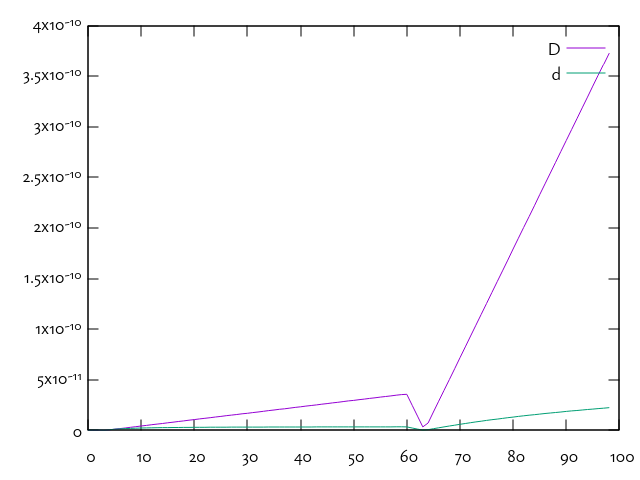
\includegraphics{Delta.png}
	% \caption{D --- абсолютна похибка, d --- відносна}

	{D --- абсолютна похибка, d --- відносна}
% \end{figure}

}

\section*{ Висновок}

\tcobx{
Обчислив суму послідовності, склавши програму мовою
Python. Зробив, щоб виводила всі дані, потрібні для формування
таблиці, та побудував графік за допомогою `gnuplot`.
}

\end{document}
